\documentclass[11pt,a4paper]{report}
\usepackage[textwidth=37em,vmargin=30mm]{geometry}
\usepackage{calc,xunicode,amsmath,amssymb,paralist,enumitem,tabu,booktabs,datetime2,xeCJK,xeCJKfntef,listings}
\usepackage{tocloft,fancyhdr,tcolorbox,xcolor,graphicx,eso-pic,xltxtra,xelatexemoji}

\newcommand{\envyear}[0]{2024}
\newcommand{\envdatestr}[0]{2024-11-16}
\newcommand{\envfinaldir}[0]{webdb/2024/20241116/final}

\usepackage[hidelinks]{hyperref}
\hypersetup{
    colorlinks=false,
    pdfpagemode=FullScreen,
    pdftitle={Web Digest - \envdatestr}
}

\setlength{\cftbeforechapskip}{10pt}
\renewcommand{\cftchapfont}{\rmfamily\bfseries\large\raggedright}
\setlength{\cftbeforesecskip}{2pt}
\renewcommand{\cftsecfont}{\sffamily\small\raggedright}

\setdefaultleftmargin{2em}{2em}{1em}{1em}{1em}{1em}

\usepackage{xeCJK,xeCJKfntef}
\xeCJKsetup{PunctStyle=plain,RubberPunctSkip=false,CJKglue=\strut\hskip 0pt plus 0.1em minus 0.05em,CJKecglue=\strut\hskip 0.22em plus 0.2em}
\XeTeXlinebreaklocale "zh"
\XeTeXlinebreakskip = 0pt


\setmainfont{Brygada 1918}
\setromanfont{Brygada 1918}
\setsansfont{IBM Plex Sans}
\setmonofont{JetBrains Mono NL}
\setCJKmainfont{Noto Serif CJK SC}
\setCJKromanfont{Noto Serif CJK SC}
\setCJKsansfont{Noto Sans CJK SC}
\setCJKmonofont{Noto Sans CJK SC}

\setlength{\parindent}{0pt}
\setlength{\parskip}{8pt}
\linespread{1.15}

\lstset{
	basicstyle=\ttfamily\footnotesize,
	numbersep=5pt,
	backgroundcolor=\color{black!5},
	showspaces=false,
	showstringspaces=false,
	showtabs=false,
	tabsize=2,
	captionpos=b,
	breaklines=true,
	breakatwhitespace=true,
	breakautoindent=true,
	linewidth=\textwidth
}






\newcommand{\coverpic}[2]{
    % argv: itemurl, authorname
    Cover photo by #2~~(\href{#1}{#1})
}
\newcommand{\makeheader}[0]{
    \begin{titlepage}
        % \newgeometry{hmargin=15mm,tmargin=21mm,bmargin=12mm}
        \begin{center}
            
            \rmfamily\scshape
            \fontspec{BaskervilleF}
            \fontspec{Old Standard}
            \fontsize{59pt}{70pt}\selectfont
            WEB\hfill DIGEST
            
            \vfill
            % \vskip 30pt
            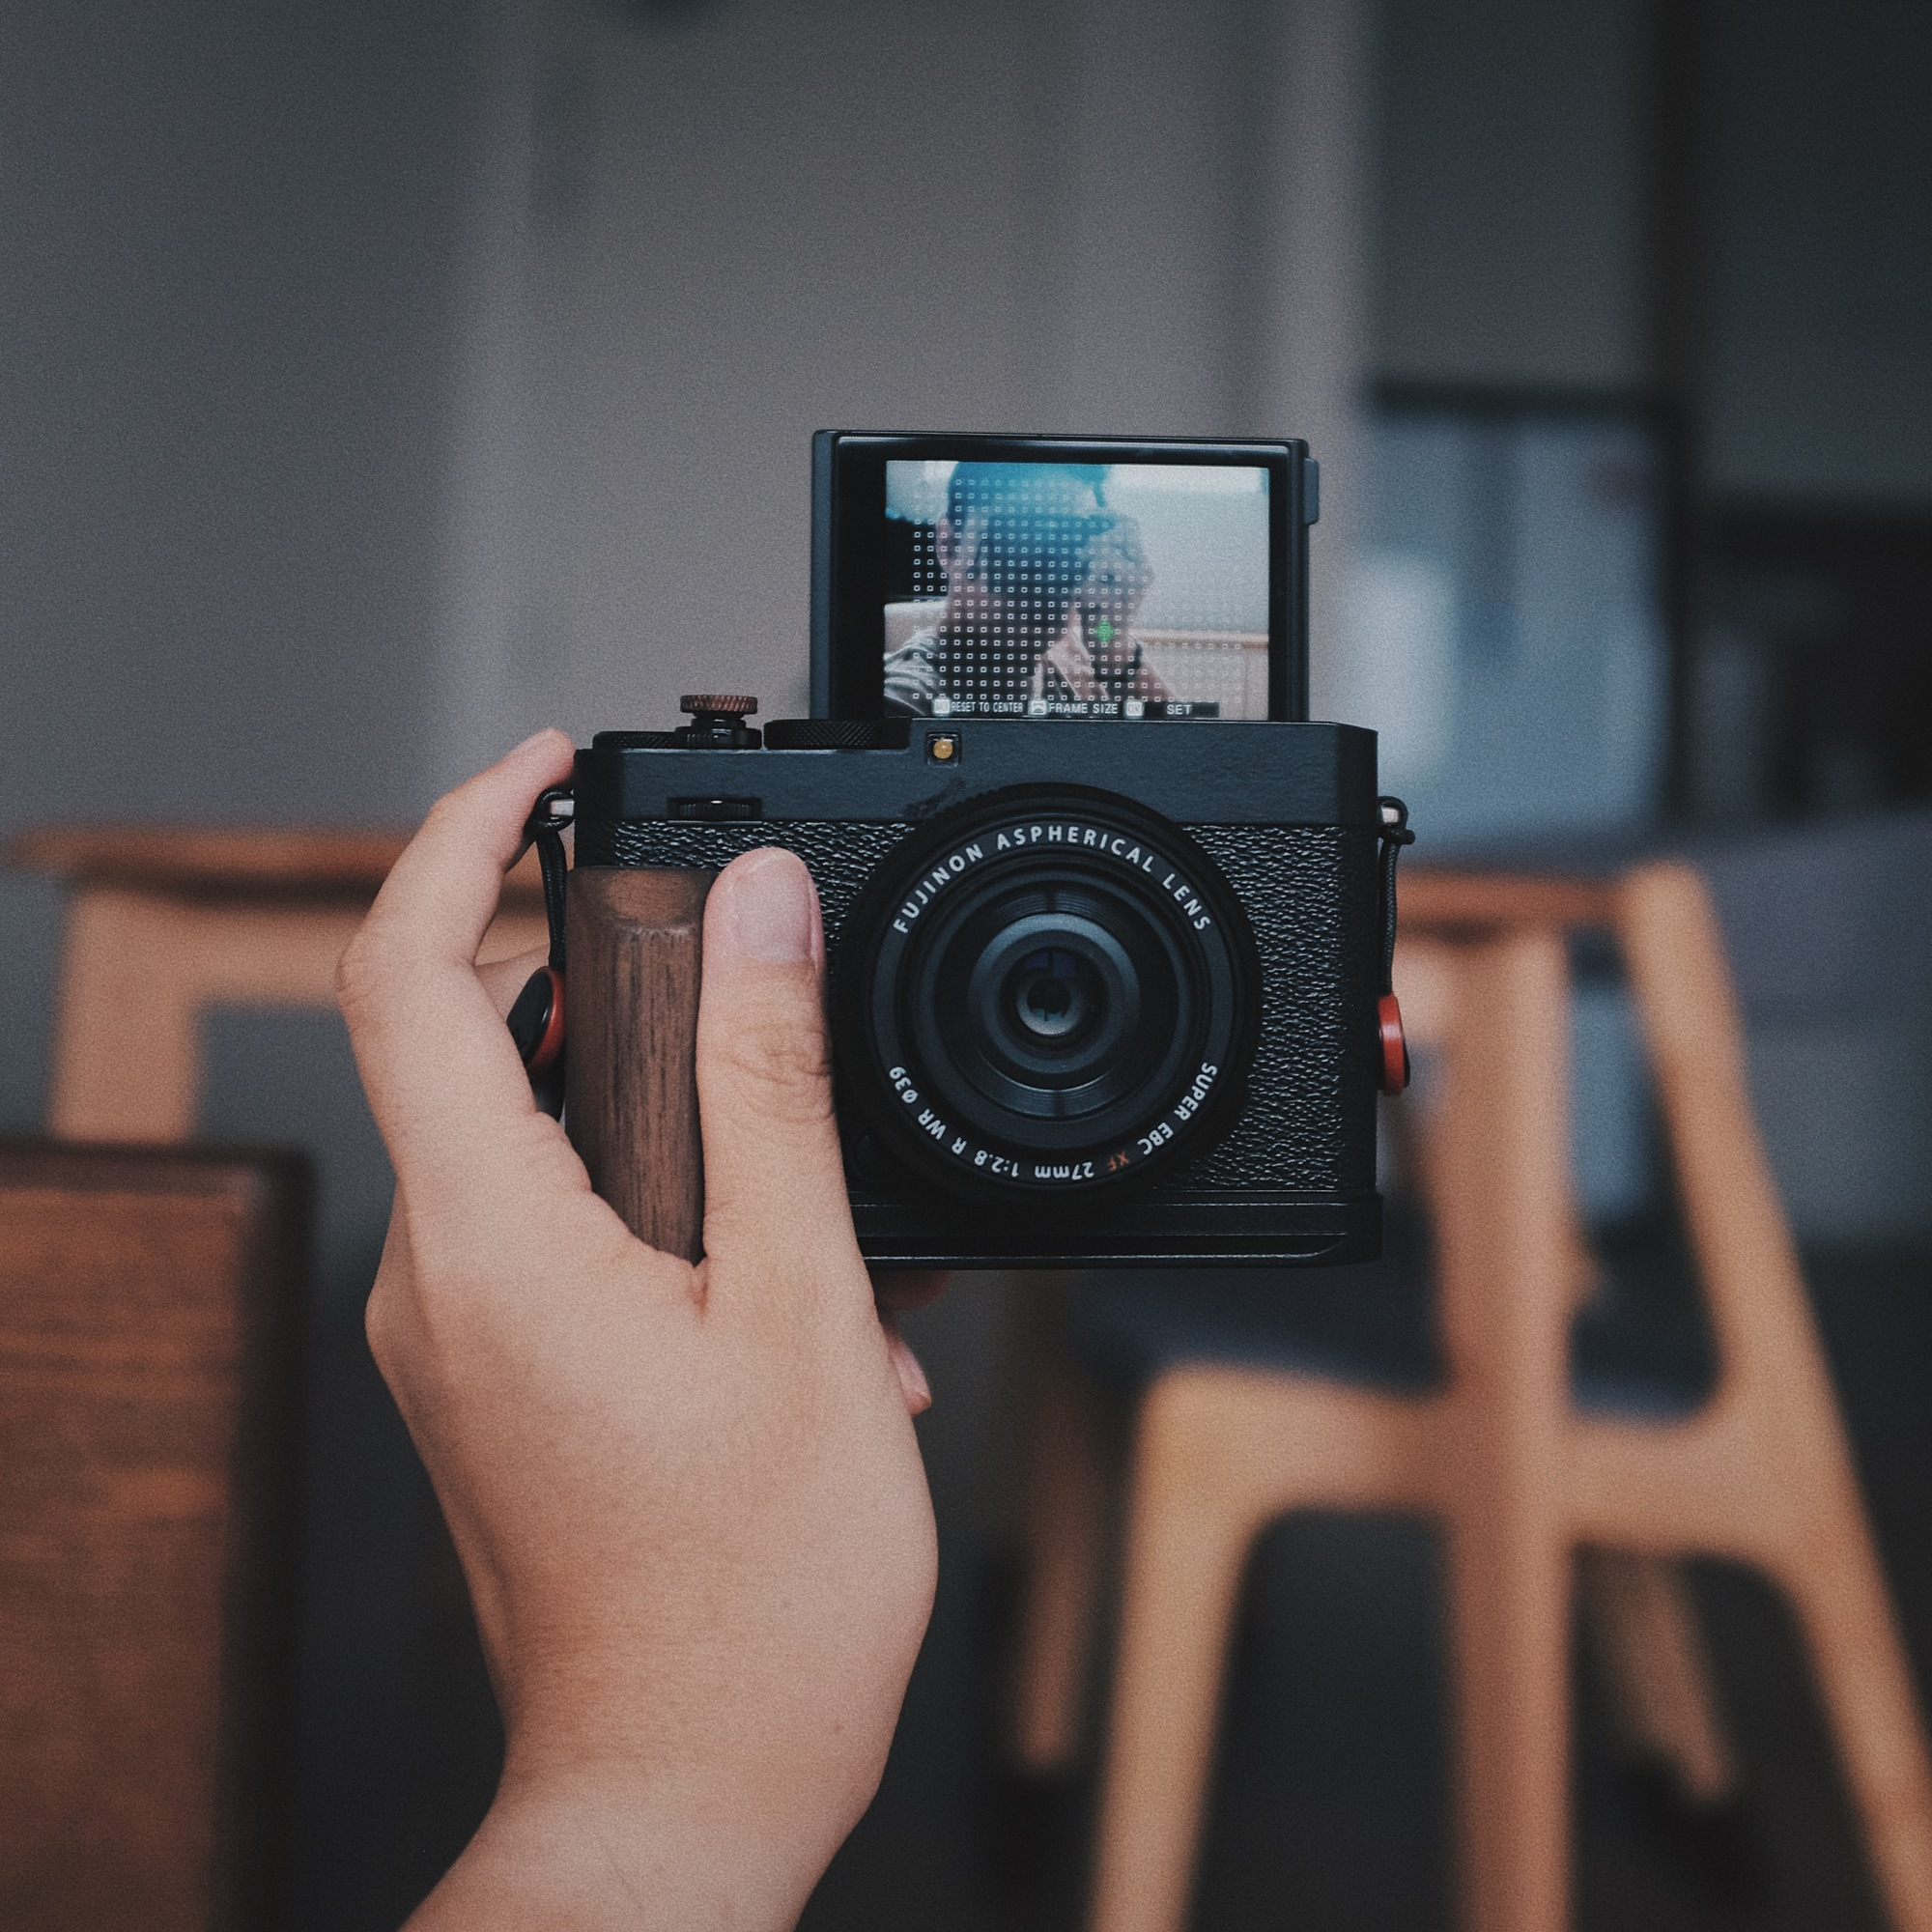
\includegraphics[width=\linewidth]{\envfinaldir/coverpic-prod.jpg}\par
            % \vskip 30pt
            \vfill

            \normalsize\rmfamily\scshape
            \copyright{} The Web Digest Project \hfill\large \envdatestr
        \end{center}
    \end{titlepage}
    % \restoregeometry
}
\newcommand{\simplehref}[1]{%
    \textcolor{blue!80!green}{\href{#1}{#1}}%
}
\renewcommand{\contentsname}{\center\Huge\sffamily\bfseries Contents\par\vskip 20pt}
\newcounter{ipartcounter}
\setcounter{ipartcounter}{0}
\newcommand{\ipart}[1]{
    % \vskip 20pt
    \clearpage
    \stepcounter{ipartcounter}
    \phantomsection
    \addcontentsline{toc}{chapter}{#1}
    % \begin{center}
    %     \Huge
    %     \sffamily\bfseries
    %     #1
    % \end{center}
    % \vskip 20pt plus 7pt
}
\newcounter{ichaptercounter}
\setcounter{ichaptercounter}{0}
\newcommand{\ichapter}[1]{
    % \vskip 20pt
    \clearpage
    \stepcounter{ichaptercounter}
    \phantomsection
    \addcontentsline{toc}{section}{\numberline{\arabic{ichaptercounter}}#1}
    \begin{center}
        \Huge
        \sffamily\bfseries
        #1
    \end{center}
    \vskip 20pt plus 7pt
}
\newcommand{\entrytitlefont}[1]{\subsection*{\raggedright\Large\sffamily\bfseries#1}}
\newcommand{\entryitemGeneric}[2]{
    % argv: title, url
    \parbox{\linewidth}{
        \entrytitlefont{#1}\par\vskip 5pt
        \footnotesize\ttfamily\mdseries
        \simplehref{#2}
    }\vskip 11pt plus 11pt minus 1pt
}
\newcommand{\entryitemGithub}[3]{
    % argv: title, url, desc
    \parbox{\linewidth}{
        \entrytitlefont{#1}\par\vskip 5pt
        \footnotesize\ttfamily\mdseries
        \simplehref{#2}\par\vskip 5pt
        \small\rmfamily\mdseries#3
    }\vskip 11pt plus 11pt minus 1pt
}
\newcommand{\entryitemAp}[3]{
    % argv: title, url, desc
    \parbox{\linewidth}{
        \entrytitlefont{#1}\par\vskip 5pt
        \footnotesize\ttfamily\mdseries
        \simplehref{#2}\par\vskip 5pt
        \small\rmfamily\mdseries#3
    }\vskip 11pt plus 11pt minus 1pt
}
\newcommand{\entryitemHackernews}[3]{
    % argv: title, hnurl, rawurl
    % \parbox{\linewidth}{
    %     \entrytitlefont{#1}\par\vskip 5pt
    %     \footnotesize\ttfamily\mdseries
    %     \simplehref{#3}\par
    %     \textcolor{black!50}{\href{#2}{#2}}
    % }\vskip 11pt plus 11pt minus 1pt
    \begin{minipage}{\linewidth}
            \entrytitlefont{#1}\par\vskip 5pt
            \footnotesize\ttfamily\mdseries
            \simplehref{#3}\par
            \textcolor{black!50}{\href{#2}{#2}}
    \end{minipage}\par\vskip 11pt plus 11pt minus 1pt
}







\begin{document}

\makeheader

\tableofcontents\clearpage




\ipart{Developers}
\ichapter{Hacker News}
\entryitemTwoLinks{Half-Life 2: 20th Anniversary Update}{https://news.ycombinator.com/item?id=42151865}{https://www.half-life.com/en/halflife2/20th}

\entryitemTwoLinks{Tesla has the highest fatal accident rate of all auto brands, study finds}{https://news.ycombinator.com/item?id=42150443}{https://www.roadandtrack.com/news/a62919131/tesla-has-highest-fatal-accident-rate-of-all-auto-brands-study/}

\entryitemTwoLinks{Maybe Bluesky has "won"}{https://news.ycombinator.com/item?id=42150278}{https://anderegg.ca/2024/11/15/maybe-bluesky-has-won}

\entryitemTwoLinks{Biological Miracle – Wood Frog}{https://news.ycombinator.com/item?id=42149433}{https://www.nps.gov/gaar/learn/nature/wood-frog-page-2.htm}

\entryitemTwoLinks{Show HN: Free mortgage analysis tool to avoid getting screwed by closing costs}{https://news.ycombinator.com/item?id=42149044}{https://closingwtf.com}

\entryitemTwoLinks{Please stop the coding challenges}{https://news.ycombinator.com/item?id=42147790}{https://blackentropy.bearblog.dev/please-stop-the-absurd-coding-challenges/}

\entryitemTwoLinks{Norwegian fishermen hunting for halibut caught a US nuclear sub}{https://news.ycombinator.com/item?id=42147675}{https://www.vice.com/en/article/fishermen-hunting-for-halibut-caught-a-us-nuclear-sub/}

\entryitemTwoLinks{The Battle Line at Louvain}{https://news.ycombinator.com/item?id=42146957}{https://www.privatdozent.co/p/the-battle-line-at-louvain-1914}

\entryitemTwoLinks{Seer: A GUI front end to GDB for Linux}{https://news.ycombinator.com/item?id=42146338}{https://github.com/epasveer/seer}

\entryitemTwoLinks{Show HN: OnAir – create link, receive calls}{https://news.ycombinator.com/item?id=42145419}{https://onair.io/}

\entryitemTwoLinks{1M people have joined Bluesky in the last day}{https://news.ycombinator.com/item?id=42144340}{https://bsky.app/profile/bsky.app/post/3lax5zxh7bc2p}

\entryitemTwoLinks{Relativty: An open-source VR headset for \$200}{https://news.ycombinator.com/item?id=42143269}{https://www.relativty.com/}

\entryitemTwoLinks{New Apple security feature reboots iPhones after 3 days, researchers confirm}{https://news.ycombinator.com/item?id=42143265}{https://techcrunch.com/2024/11/14/new-apple-security-feature-reboots-iphones-after-3-days-researchers-confirm/}

\entryitemTwoLinks{Are We PEP740 Yet?}{https://news.ycombinator.com/item?id=42142864}{https://trailofbits.github.io/are-we-pep740-yet/}

\entryitemTwoLinks{Matrix Client Tutorial}{https://news.ycombinator.com/item?id=42142790}{https://uhoreg.gitlab.io/matrix-tutorial/index.html}

\entryitemTwoLinks{Analysis of economic and productivity losses caused by cookie banners in Europe}{https://news.ycombinator.com/item?id=42141843}{https://legiscope.com/blog/hidden-productivity-drain-cookie-banners.html}

\entryitemTwoLinks{Thomas E. Kurtz has died}{https://news.ycombinator.com/item?id=42141761}{https://computerhistory.org/blog/in-memoriam-thomas-e-kurtz-1928-2024/}

\entryitemTwoLinks{Visual Basic 6 IDE recreated in C\#}{https://news.ycombinator.com/item?id=42141587}{https://github.com/BAndysc/AvaloniaVisualBasic6}

\entryitemTwoLinks{Old Vintage Computing Research: Dusting Off Dreamcast Linux}{https://news.ycombinator.com/item?id=42140863}{http://oldvcr.blogspot.com/2023/02/dusting-off-dreamcast-linux.html}

\entryitemTwoLinks{Speeding up the Rust edit-build-run cycle}{https://news.ycombinator.com/item?id=42140164}{https://davidlattimore.github.io/posts/2024/02/04/speeding-up-the-rust-edit-build-run-cycle.html}\ichapter{Phoronix}
\entryitemGeneric{\hskip 0pt{}Tmpfs Adding Case Insensitive Support For Wine / Steam Play \& Flatpaks}{https://www.phoronix.com/news/Linux-6.13-Tmpfs-Case-Folding}

\entryitemGeneric{\hskip 0pt{}Linux 6.13 To Expand Atomic Write Support To EXT4 \& XFS}{https://www.phoronix.com/news/Linux-6.13-VFS-Untorn-Writes}

\entryitemGeneric{\hskip 0pt{}Linux 6.13 Very Exciting With New Feature Code For AMD EPYC Zen 5, Intel Panther Lake}{https://www.phoronix.com/news/Linux-6.13-Features-Early}

\entryitemGeneric{\hskip 0pt{}GNOME Mutter Switches To High Priority KMS Thread To Avoid Crashes}{https://www.phoronix.com/news/GNOME-High-Priority-KMS-Thread}

\entryitemGeneric{\hskip 0pt{}Linux 6.12 Preps For Release With Real-Time, Sched\_Ext, Stable Xe2 \& Raspberry Pi 5}{https://www.phoronix.com/news/Linux-6.12-Feature-Reminder}

\entryitemGeneric{\hskip 0pt{}Google Posts Patches Further Speeding Up Linux Async Device Suspend \& Resume}{https://www.phoronix.com/news/Faster-Async-Suspend-Resume}

\entryitemGeneric{\hskip 0pt{}AMD Releases ZenDNN 5.0 For Deep Neural Network Library Optimized For Zen 5 EPYC}{https://www.phoronix.com/news/AMD-ZenDNN-5.0-Released}

\entryitemGeneric{\hskip 0pt{}GCC 15 Adds Option For Arm Guarded Control Stack "GCS" Code Generation}{https://www.phoronix.com/news/GCC-15-Arm-GCS-Code-Generation}

\entryitemGeneric{\hskip 0pt{}Linux Patches Add Support For New "Phone Link" Hotkey On Latest ThinkPads}{https://www.phoronix.com/news/Linux-Phone-Link-Hotkey}


\ipart{Developers~~~~(zh-Hans)}
\ichapter{Solidot}
\entryitemGeneric{\hskip 0pt{}Yandex 禁止中国 IP 搜索图片和视频}{https://www.solidot.org/story?sid=79791}

\entryitemGeneric{\hskip 0pt{}调查显示 AI 热在降温}{https://www.solidot.org/story?sid=79790}

\entryitemGeneric{\hskip 0pt{}OpenAI、Google 和 Anthropic 在构建更先进 AI 模型上遭遇瓶颈}{https://www.solidot.org/story?sid=79789}

\entryitemGeneric{\hskip 0pt{}网信办发布《移动互联网未成年人模式建设指南》}{https://www.solidot.org/story?sid=79788}

\entryitemGeneric{\hskip 0pt{}《半条命2》迎来二十周年,社区开发者制作 RTX 版本}{https://www.solidot.org/story?sid=79787}

\entryitemGeneric{\hskip 0pt{}美团单车和哈啰单车在郑州市暂停运营}{https://www.solidot.org/story?sid=79786}

\entryitemGeneric{\hskip 0pt{}研究发现错过截止日期会导致他人更苛刻的评价你的工作}{https://www.solidot.org/story?sid=79785}

\entryitemGeneric{\hskip 0pt{}美国黑客因窃取 Bitfinex 比特币被判五年}{https://www.solidot.org/story?sid=79784}

\entryitemGeneric{\hskip 0pt{}中国的机器人革命迫使劳动力作出改变}{https://www.solidot.org/story?sid=79783}

\entryitemGeneric{\hskip 0pt{}韩国研究人员重新发明轮子}{https://www.solidot.org/story?sid=79782}

\entryitemGeneric{\hskip 0pt{}OpenMP 6.0 释出}{https://www.solidot.org/story?sid=79781}

\entryitemGeneric{\hskip 0pt{}Meta 因违反欧盟反垄断规定被罚 8.4 亿美元}{https://www.solidot.org/story?sid=79780}

\entryitemGeneric{\hskip 0pt{}因使用盗版软件期刊撤下了两篇论文}{https://www.solidot.org/story?sid=79779}

\entryitemGeneric{\hskip 0pt{}洋葱新闻拍下了 InfoWars}{https://www.solidot.org/story?sid=79778}

\entryitemGeneric{\hskip 0pt{}意大利出人意料的成为间谍软件的主要供应国}{https://www.solidot.org/story?sid=79777}

\entryitemGeneric{\hskip 0pt{}AI 只能完成高等数学新测试问题的不到 2\%}{https://www.solidot.org/story?sid=79776}

\entryitemGeneric{\hskip 0pt{}GOG 宣布了经典游戏的保存计划}{https://www.solidot.org/story?sid=79775}

\entryitemGeneric{\hskip 0pt{}Steam 停止支持 Windows 7 和 Windows 8}{https://www.solidot.org/story?sid=79774}

\entryitemGeneric{\hskip 0pt{}微软证实在开发掌机}{https://www.solidot.org/story?sid=79773}

\entryitemGeneric{\hskip 0pt{}微软宣布 .NET 9}{https://www.solidot.org/story?sid=79772}\ichapter{V2EX}
\entryitemGeneric{\hskip 0pt{}[互联网] Linux .do 的邀请咸鱼竟然值 50,那么贵?}{https://www.v2ex.com/t/1090011}

\entryitemGeneric{\hskip 0pt{}[职场话题] 工作内耗和自我折磨}{https://www.v2ex.com/t/1090010}

\entryitemGeneric{\hskip 0pt{}[随想] 身边有不少朋友一辈子不上班也过得很开心}{https://www.v2ex.com/t/1090009}

\entryitemGeneric{\hskip 0pt{}[Apple] 抢了台 Macmini m4+24+512+10G 补贴后挺香的}{https://www.v2ex.com/t/1090008}

\entryitemGeneric{\hskip 0pt{}[天黑以后] 20241116 午夜俱乐部}{https://www.v2ex.com/t/1090007}

\entryitemGeneric{\hskip 0pt{}[VPS] 监测 VPS 线路情况}{https://www.v2ex.com/t/1090006}

\entryitemGeneric{\hskip 0pt{}[北京] 想买一只黑柴犬,北京或者周边哪里合适?}{https://www.v2ex.com/t/1090005}

\entryitemGeneric{\hskip 0pt{}[程序员] 产品经理的第一个开源项目: ClipShare-让网页内容分享更优雅}{https://www.v2ex.com/t/1090003}

\entryitemGeneric{\hskip 0pt{}[投资] 感觉大的要来了}{https://www.v2ex.com/t/1090002}

\entryitemGeneric{\hskip 0pt{}[程序员] 求推荐效果好的数字人服务}{https://www.v2ex.com/t/1090001}

\entryitemGeneric{\hskip 0pt{}[宽带症候群] Apple 专卖店的网络, Guest Wi-Fi 和 Demo 都一样}{https://www.v2ex.com/t/1090000}

\entryitemGeneric{\hskip 0pt{}[问与答] Bark 是不是换开发者了?印象中之前不是黄丰,最近更新很频繁还刚刚加了捐赠,更新日志风格也和之前不太一样}{https://www.v2ex.com/t/1089999}

\entryitemGeneric{\hskip 0pt{}[VPS] 今天墙变高了吗,自建节点被墙了}{https://www.v2ex.com/t/1089998}

\entryitemGeneric{\hskip 0pt{}[问与答] 老哥们,关于是否购买学区房想跟大家讨论一下}{https://www.v2ex.com/t/1089997}

\entryitemGeneric{\hskip 0pt{}[问与答] 有谁知道极客湾的这个视频里用到的 usb 电流计是什么牌子的吗?我想买一个同款的}{https://www.v2ex.com/t/1089995}

\entryitemGeneric{\hskip 0pt{}[Apple] mac mini 10g 补货了}{https://www.v2ex.com/t/1089994}

\entryitemGeneric{\hskip 0pt{}[AirPods] Airpods Pro 总是自动断连我的 Mac Mini M4, 可能的原因是啥?}{https://www.v2ex.com/t/1089991}

\entryitemGeneric{\hskip 0pt{}[程序员] Distributer - 免费内容分发的效率之选}{https://www.v2ex.com/t/1089989}

\entryitemGeneric{\hskip 0pt{}[Telegram] telegram api 是不是现在不能申请了,一直返回 error 有无代申请的,有偿~}{https://www.v2ex.com/t/1089988}

\entryitemGeneric{\hskip 0pt{}[Apple] 笑死,国补买成 m2 了,不能退了}{https://www.v2ex.com/t/1089987}

\entryitemGeneric{\hskip 0pt{}[问与答] 有没有买了 m4pro 的朋友?}{https://www.v2ex.com/t/1089986}

\entryitemGeneric{\hskip 0pt{}[RSS] 请问 Follow 的视频订阅怎么把视频框调大一点?}{https://www.v2ex.com/t/1089984}

\entryitemGeneric{\hskip 0pt{}[分享创造] 从零基础到上线 AI 图像编辑网站,我的 2 小时"极速 startup"记录 🚀}{https://www.v2ex.com/t/1089983}

\entryitemGeneric{\hskip 0pt{}[macOS] M1 Pro 上最好将部分 App 放入沙盒运行的办法是什么}{https://www.v2ex.com/t/1089982}

\entryitemGeneric{\hskip 0pt{}[程序员] 把推特当博客和笔记如何?}{https://www.v2ex.com/t/1089981}

\entryitemGeneric{\hskip 0pt{}[程序员] 请教下游戏前端面试是否要刷 Leetcode?}{https://www.v2ex.com/t/1089980}

\entryitemGeneric{\hskip 0pt{}[Apple] 夜间充电自动化开关 QX,优化暂停充电时遇到 BUG}{https://www.v2ex.com/t/1089979}

\entryitemGeneric{\hskip 0pt{}[English] 大佬们,词根词缀法记单词是真的有用吗?}{https://www.v2ex.com/t/1089978}

\entryitemGeneric{\hskip 0pt{}[NAS] 求一个 MoviePilot 认证站点}{https://www.v2ex.com/t/1089977}

\entryitemGeneric{\hskip 0pt{}[酷工作] Position : ZK Engineer(Remote/Web3)}{https://www.v2ex.com/t/1089976}

\entryitemGeneric{\hskip 0pt{}[分享发现] 安卓的 B 站 App,长按倍速播放的时候,播放效果和 iOS 不一样}{https://www.v2ex.com/t/1089975}

\entryitemGeneric{\hskip 0pt{}[Apple] Apple Music 家庭版有两个位置谁来}{https://www.v2ex.com/t/1089973}

\entryitemGeneric{\hskip 0pt{}[问与答] 用内地手机号拨打境外号码会触发反诈吗?}{https://www.v2ex.com/t/1089972}

\entryitemGeneric{\hskip 0pt{}[程序员] v2ex 是怎么做到 seo 这么牛逼的}{https://www.v2ex.com/t/1089970}

\entryitemGeneric{\hskip 0pt{}[OpenWrt] OpenWrt 切换至 apk 包管理器}{https://www.v2ex.com/t/1089968}

\entryitemGeneric{\hskip 0pt{}[分享发现] 分享:马斯克 xAI Grok-2 申请 API,赠送 25 美金}{https://www.v2ex.com/t/1089967}

\entryitemGeneric{\hskip 0pt{}[Android] 三星 OneUI 有办法在插非+86 SIM 卡的情况下用国区应用商店吗?}{https://www.v2ex.com/t/1089966}

\entryitemGeneric{\hskip 0pt{}[分享发现] 为啥越来越觉得 bing 搜索不太行…}{https://www.v2ex.com/t/1089965}

\entryitemGeneric{\hskip 0pt{}[VXNA] 申请收录博客: Xie Yonglin}{https://www.v2ex.com/t/1089964}

\entryitemGeneric{\hskip 0pt{}[分享发现] Wildcard 也难逃被 Claude 封号的命运}{https://www.v2ex.com/t/1089962}

\entryitemGeneric{\hskip 0pt{}[分享发现] Google SEO 关键词新词挖掘并不神秘,别人几千一年才教你的东西我免费告诉你}{https://www.v2ex.com/t/1089961}

\entryitemGeneric{\hskip 0pt{}[问与答] 想问一下大家,小区车位临停收费比周边商场还贵,这事儿有解吗?}{https://www.v2ex.com/t/1089960}

\entryitemGeneric{\hskip 0pt{}[职场话题] 降薪了,工作六年麻木了}{https://www.v2ex.com/t/1089959}

\entryitemGeneric{\hskip 0pt{}[问与答] 搬新家,开发商配的 AC+AP 网络,可以用路由器替换 AP 面板吗?}{https://www.v2ex.com/t/1089958}

\entryitemGeneric{\hskip 0pt{}[问与答] 外企工作中,``移除了部分收件人''的提醒在邮件中怎样用英文表达比较地道?}{https://www.v2ex.com/t/1089957}

\entryitemGeneric{\hskip 0pt{}[全球工单系统] 抖音验证码登录居然要求实名人脸认证!}{https://www.v2ex.com/t/1089955}

\entryitemGeneric{\hskip 0pt{}[macOS] 屏幕被全局上了文字水印,怎么排查?}{https://www.v2ex.com/t/1089954}

\entryitemGeneric{\hskip 0pt{}[问与答] Mac 意外重启后 iTerm2 所有窗口都没了,有没有人有经验能救回来?}{https://www.v2ex.com/t/1089953}

\entryitemGeneric{\hskip 0pt{}[问与答] 迄今为止,你最喜欢的一句话是什么?}{https://www.v2ex.com/t/1089952}

\entryitemGeneric{\hskip 0pt{}[服务器] 服务器机柜 如何规划摆放顺序?}{https://www.v2ex.com/t/1089951}


\ipart{Generic News}
\ichapter{Reuters}
\entryitemWithDescription{\hskip 0pt{}Dutch government crisis defused, prime minister says}{https://www.reuters.com/world/europe/dutch-government-crisis-defused-prime-minister-says-2024-11-15/}{A government crisis in the Netherlands was avoided in a tense emergency meeting on Friday, as a cabinet member resigned over the government\textquotesingle s handling of violence involving fans of an Israeli soccer team in Amsterdam last...}

\entryitemWithDescription{\hskip 0pt{}German project reinvents 1884 Berlin Conference to mull legacy of colonialism}{https://www.reuters.com/world/german-project-reinvents-1884-berlin-conference-mull-legacy-colonialism-2024-11-15/}{Activists, artists and academics brought together by German cultural project Dekoloniale gathered in Berlin on Friday, 140 years after European leaders divided up the African continent between them, to discuss the legacy of colonialism...}

\entryitemWithDescription{\hskip 0pt{}Russian air defences down Ukrainian drones in different regions}{https://www.reuters.com/world/europe/russian-air-defences-down-ukrainian-drones-different-regions-2024-11-15/}{Russian air defence units intercepted a series of Ukrainian drones in several Russian regions, officials said, many of them in Kursk region, where Ukrainian troops launched a major incursion in...}

\entryitemWithDescription{\hskip 0pt{}Iran backs Lebanon in ceasefire talks, seeks end to 'problems'}{https://www.reuters.com/world/middle-east/israel-hits-beirut-suburb-after-us-delivers-truce-proposal-2024-11-15/}{Iran backs any decision taken by Lebanon in talks to secure a ceasefire with Israel, a senior Iranian official said on Friday, signalling Tehran wants to see an end to a conflict that has dealt heavy blows to its Lebanese ally...}

\entryitemWithDescription{\hskip 0pt{}In echo of Soviet era, Russians are informing on each other over Ukraine}{https://www.reuters.com/world/europe/more-russians-denounce-each-other-over-ukraine-echo-soviet-era-2024-11-15/}{Critics say the wave of denunciations is helping President Vladimir Putin\textquotesingle s government crack down on...}

\entryitemWithDescription{\hskip 0pt{}Germany's Scholz calls Putin, ending Western isolation over Ukraine}{https://www.reuters.com/world/europe/germanys-scholz-russias-putin-hold-phone-call-friday-bloomberg-reports-2024-11-15/}{Olaf Scholz spoke with Vladimir Putin on Friday for the first time in nearly two...}

\entryitemWithDescription{\hskip 0pt{}Biden meets South Korea, Japan leaders for pre-Trump huddle on risk}{https://www.reuters.com/world/biden-meet-south-korea-japan-leaders-pre-trump-huddle-risk-2024-11-15/}{U.S. President Joe Bidenmet with Japan and South Korea\textquotesingle s leaders on Friday as they sought to cement their diplomatic progress ahead of a new Trump administration that many fear could upend alliances...}

\entryitemWithDescription{\hskip 0pt{}Le Pen allies decry witch-hunt as prosecutors threaten her French presidential hopes}{https://www.reuters.com/world/europe/le-pen-allies-decry-witch-hunt-prosecutors-threaten-her-french-presidential-2024-11-15/}{Allies of French far-right leader Marine Le Pen have accused the judiciary of a witch hunt and undue meddling in democracy after prosecutors requested she face an obligatory five-year ban from public office if convicted of misusing...}

\entryitemWithDescription{\hskip 0pt{}Austria says Russia to cut off gas from Saturday}{https://www.reuters.com/markets/commodities/austrias-omv-informed-by-gazprom-that-deliveries-be-reduced-0-says-platform-2024-11-15/}{Russia told Austria on Friday it will suspend gas deliveries via Ukraine on Saturday, in a development that signals a fast-approaching end of Moscow\textquotesingle s last gas flows to...}

\entryitemWithDescription{\hskip 0pt{}Protesters demand leader's ouster in Russian-backed breakaway region of Georgia}{https://www.reuters.com/world/europe/protests-erupt-outside-parliament-breakaway-georgian-region-tass-says-2024-11-15/}{Protesters stormed the parliament of the Russian-backed breakaway Georgian region of Abkhazia on Friday and demanded the resignation of its leader over an unpopular investment agreement with...}

\entryitemWithDescription{\hskip 0pt{}Dutch government could fall over handling of Amsterdam violence, media report}{https://www.reuters.com/world/europe/dutch-government-could-fall-over-handling-amsterdam-violence-media-report-2024-11-15/}{The Dutch cabinet met in emergency session on Friday amid reports the coalition could implode over the government\textquotesingle s handling of violence last week involving fans of an Israeli team visiting for a Europa League soccer...}

\entryitemWithDescription{\hskip 0pt{}Ukraine's Zelenskiy says Scholz-Putin phone call opens 'Pandora's box'}{https://www.reuters.com/world/europe/ukraines-zelenskiy-warned-scholz-against-putin-call-kyiv-source-says-2024-11-15/}{President Volodymyr Zelenskiy said the German chancellor\textquotesingle s phone call with Russia\textquotesingle s leader on Friday opened a "Pandora\textquotesingle s box" that undermined efforts to isolate Vladimir Putin and end the...}

\entryitemWithDescription{\hskip 0pt{}Germany's Scholz speaks with Putin in first contact since Dec 2022}{https://www.reuters.com/world/europe/germanys-scholz-speaks-with-putin-first-contact-since-dec-2022-2024-11-15/}{German Chancellor Olaf Scholz and Russian President Vladimir Putin spoke on the phone for an hour on Friday afternoon, a German government source said on...}






\clearpage
\leavevmode\vfill
\footnotesize

Copyright \copyright{} 2023-2024 Neruthes and other contributors.

This document is published with CC BY-NC-ND 4.0 license.

The entries listed in this newsletter may be copyrighted by their respective creators.

This newsletter is generated by the Web Digest project.

The newsletters are also delivered via Telegram channel \CJKunderline{\href{https://t.me/webdigestchannel}{https://t.me/webdigestchannel}}.\\
RSS feed is available at \CJKunderline{\href{https://webdigest.pages.dev/rss.xml}{https://webdigest.pages.dev/rss.xml}}.

This newsletter is available in PDF at
\CJKunderline{\href{https://webdigest.pages.dev/}{https://webdigest.pages.dev/}}.

The source code being used to generate this newsletter is available at\\
\CJKunderline{\href{https://github.com/neruthes/webdigest}{https://github.com/neruthes/webdigest}}.

This newsletter is also available in
\CJKunderline{\href{http://webdigest.pages.dev/readhtml/\envyear/WebDigest-20241116.html}{HTML}} and
\CJKunderline{\href{https://github.com/neruthes/webdigest/blob/master/markdown/\envyear/WebDigest-20241116.md}{Markdown}}.


\coverpic{https://unsplash.com/photos/a-bar-with-a-bunch-of-bottles-on-the-wall-1DsOBU6O-v0}{Mindspace Studio}


\end{document}
